% ===================================================================
% SKILL: KAPANIŞ VE KAYNAKÇA TASARIMI
% ===================================================================
% TANIM:
% Bu dosya, sunumun sonunda yer alması gereken standart kapanış 
% bölümünü içerir. İki farklı kaynakça yöntemi ve kapanış sayfasını kapsar:
% 
% 1. YÖNTEM A (Manuel): Kaynakların elle madde (item) olarak yazıldığı liste.
%    Az sayıda kaynak için uygundur.
% 
% 2. YÖNTEM B (Otomatik): BibLaTeX ve references.bib dosyasını kullanan yapı.
%    Standart şablon kullanımında önerilen yöntemdir.
% 
% 3. İLETİŞİM (Kapanış): Çift QR kodlu, "plain" (sade) formatta
%    hazırlanmış standart teşekkür ve iletişim sayfasıdır.
% ===================================================================

% -------------------------------------------------------------------
% 1. YÖNTEM A: MANUEL KAYNAKÇA LİSTESİ (Örnek)
% -------------------------------------------------------------------
% NOT: Eğer .bib dosyası kullanmıyorsanız bu bloğu kullanın.
\section{Kaynaklar (Manuel)}

\begin{frame}{Referanslar}
    \begin{itemize}
        % Kitap Referansı Örneği
        \item Walpole, R. E., Myers, R. H., Myers, S. L., \& Ye, K. (2016). \textit{Probability and Statistics for Engineers and Scientists} (9th ed.). Pearson.
        
        % Kitap Referansı Örneği 2
        \item Montgomery, D. C., \& Runger, G. C. (2018). \textit{Applied Statistics and Probability for Engineers} (7th ed.). Wiley.
        
        % Makale/Yayın Referansı Örneği
        \item Wald, A. (1943). \textit{A Method of Estimating Plane Vulnerability Based on Damage of Survivors}. Columbia University.
        
        % Ders Notu Referansı Örneği
        \item Prof.\ Dr.~Halil Rıdvan ÖZ ders notları
    \end{itemize}
\end{frame}

% -------------------------------------------------------------------
% 2. YÖNTEM B: OTOMATİK KAYNAKÇA (BibLaTeX)
% -------------------------------------------------------------------
% NOT: Şablondaki references.bib dosyasını kullanır.
% Bu yöntemin çalışması için preamble'da \addbibresource{references.bib} olmalıdır.
\section{Kaynaklar (BibLaTeX)}

% [allowframebreaks] kaynakçanın birden fazla sayfaya yayılmasını sağlar.
% Bu tek istisna olup lutbeamer kurallarına uygundur.
\begin{frame}[allowframebreaks]{Kaynaklar}
    % \nocite{*} komutu, metin içinde atıf yapılmasa bile .bib dosyasındaki
    % TÜM kaynakların listelenmesini sağlar. Sadece atıf yapılanları
    % göstermek istiyorsanız bu satırı silin.
    \nocite{*} 
    
    \printbibliography{}
\end{frame}

% -------------------------------------------------------------------
% 3. İLETİŞİM VE KAPANIŞ SAYFASI
% -------------------------------------------------------------------
\section{İletişim}
% [plain] parametresi üst/alt bilgileri (tarih, sayfa no vb.) gizler.
% Görselin odak noktası olması için kullanılır.
\begin{frame}[plain]
    \begin{center}
        % Görsel, sayfaya tam sığacak şekilde ayarlanmıştır.
        % height=0.9\textheight ile dikey taşma engellenir.
        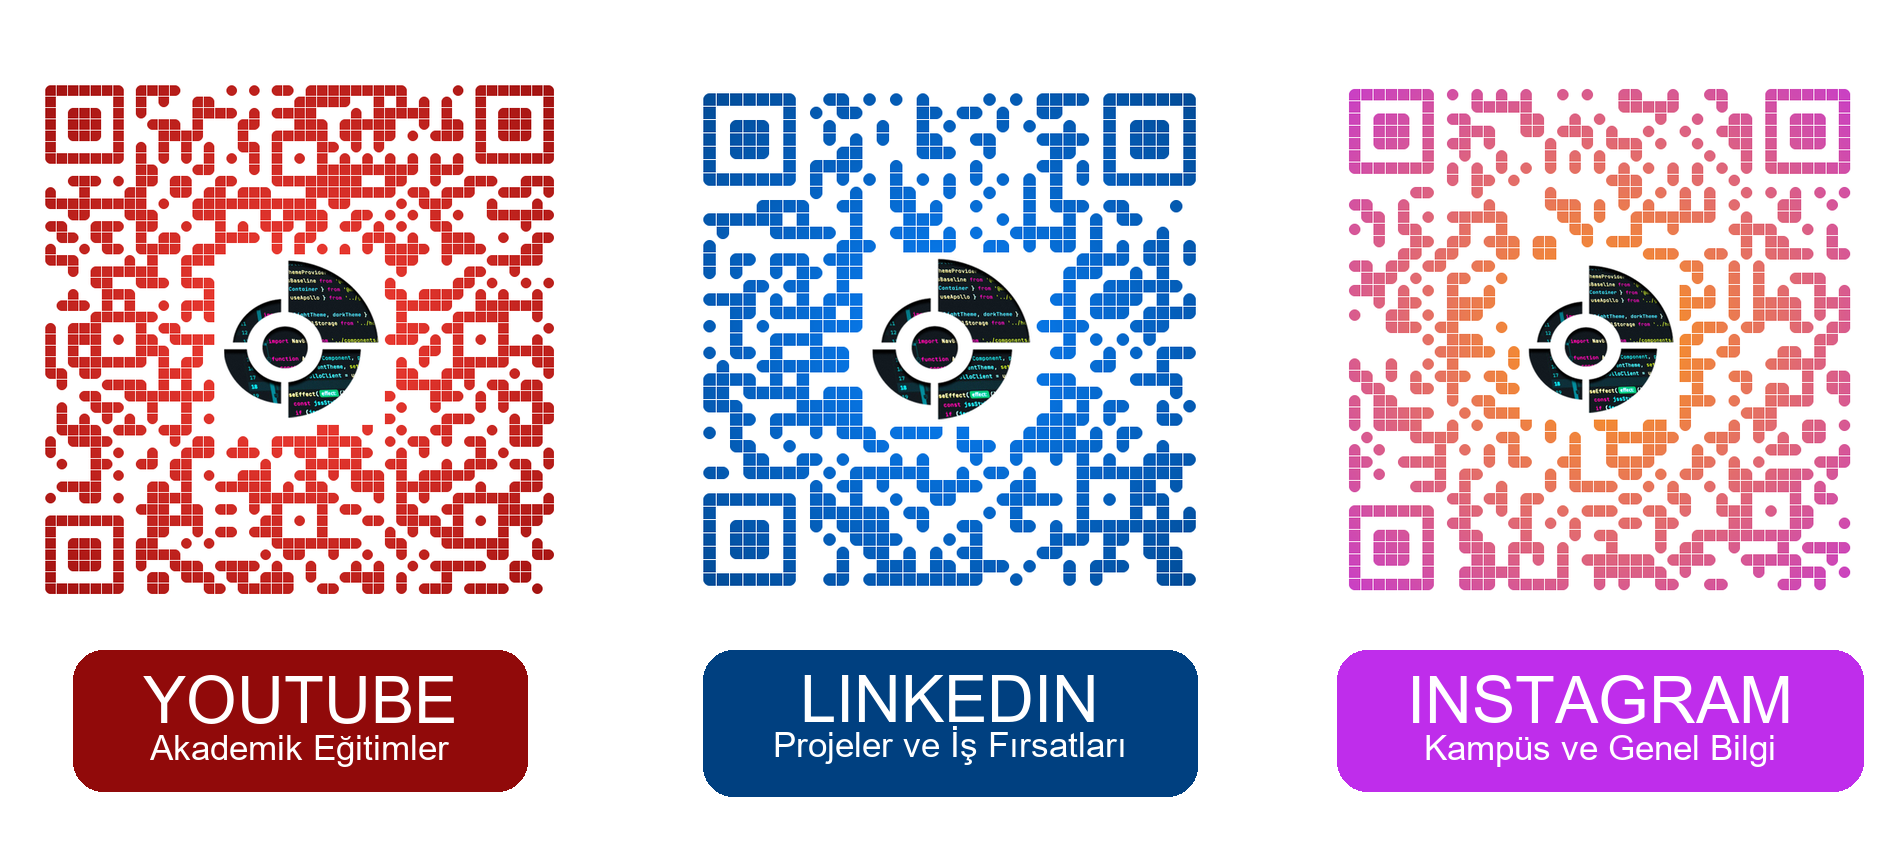
\includegraphics[width=\textwidth,height=0.9\textheight,keepaspectratio]{figures/combined_qrs.png}
    \end{center}
\end{frame}
